\begin{frame}
    \frametitle{About me}
    \begin{columns}
        \column[t]{5cm}
        \begin{itemize}
            \item Advanced Reactors and Fuel Cycles group at UIUC
            \item Software tools for development, verification, and lisencing of advanced reactors
            \item Open source
        \end{itemize}
        
        \column[t]{5cm}
        \begin{figure}[htpb]
            \centering
            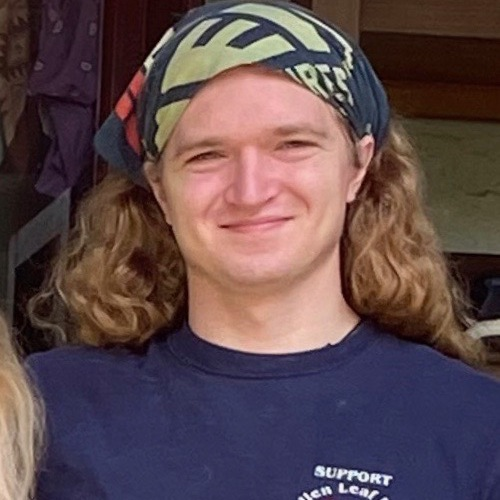
\includegraphics[width=5cm]{images/yardaso.jpeg}
        \end{figure}

    \end{columns}
\end{frame}

\begin{frame}
  \frametitle{What is software?}
  \begin{figure}[htpb]
      \centering
      \begin{subfigure}
        \centering
        
\includegraphics[width=1.5cm]{images/firefox-logo.eps}
      \end{subfigure}
      \begin{subfigure}
        \centering
        
\includegraphics[width=5cm]{images/openmc-logo.eps}
      \end{subfigure}
      \begin{subfigure}
        \centering
        
\includegraphics[width=2cm]{images/git-logo.eps}
      \end{subfigure}
  \end{figure}
  \begin{center}
    {\tiny Sources: \cite{firefox_logo}, \cite{openmc_logo}, \cite{git_logo}}
  \end{center}
  % a comment
  % add photos of software
  % firefox, openmc, etc
  \pause\medskip
  \begin{itemize}
      \item Ultimately, software is a {\it tool} we can use to solve complex problems.
  \end{itemize}
\end{frame}

\begin{frame}
    \frametitle{What kinds of problems do {\it we} use software to solve?}

    \begin{figure}[htpb]
        \begin{subfigure}
            \centering
            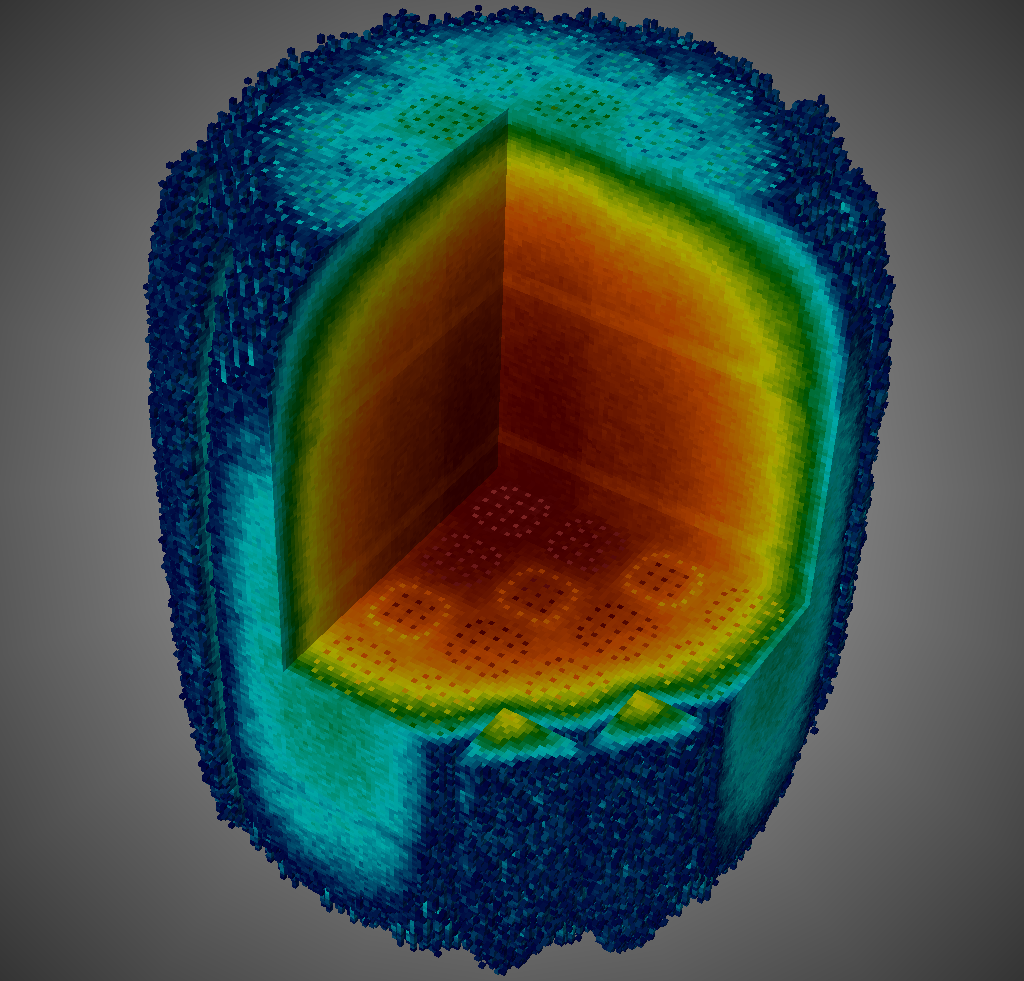
\includegraphics[width=2cm]{images/exasmr.png}
        \end{subfigure}
        \begin{subfigure}
           \centering
           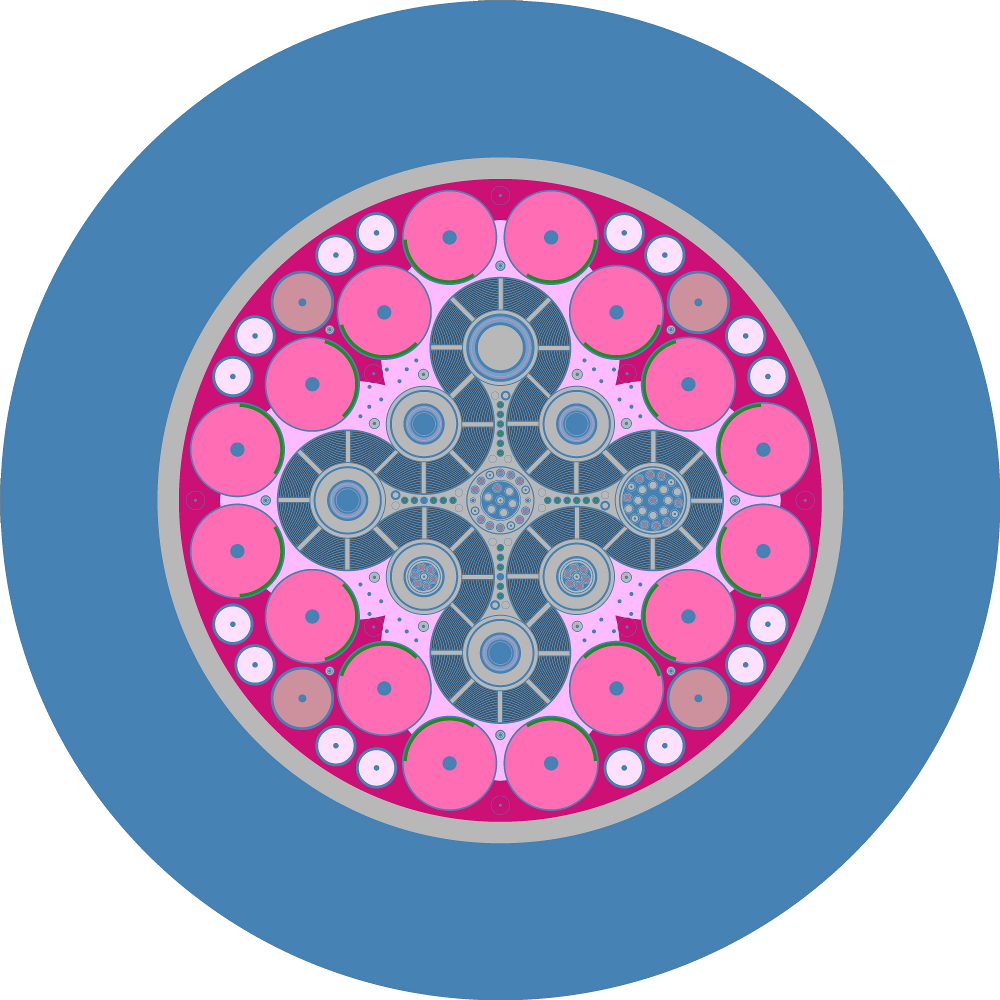
\includegraphics[width=2cm]{images/atr.png} 
        \end{subfigure}
        \begin{subfigure}
           \centering
           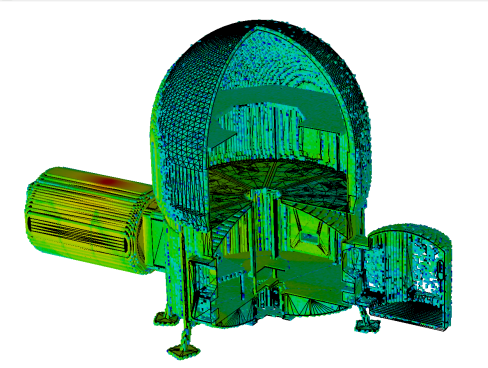
\includegraphics[width=2cm]{images/hab1.png} 
        \end{subfigure}
        \begin{subfigure}
            \centering
            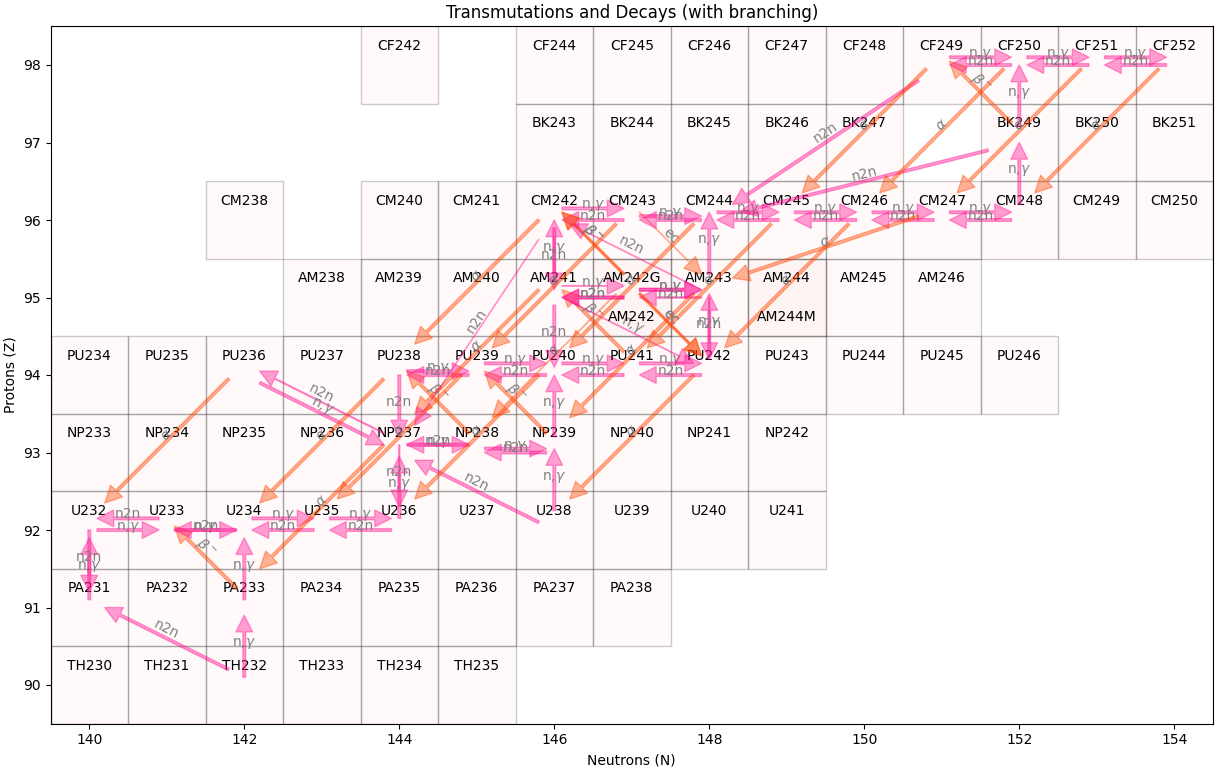
\includegraphics[width=4cm]{images/transmutation.png}
        \end{subfigure}
    \end{figure}
    \begin{center}
      {\tiny Sources: \cite{exasmr_fig},\cite{openmc_atr_slice},\cite{dagmc_nasa_module},\cite{armi_transmutation_fig}}
    \end{center}
    \pause\medskip
    \begin{itemize}
        \item Neutron transport
        \item Decay chains
        \item Materials
        \item Thermal hydraulics
        \item PRA
        \item Accident analysis
        \item {\bf Licensing activities}
    \end{itemize}

\end{frame}

\begin{frame}
    \frametitle{Open source software}
    Software whose source code is public.
    
    \begin{columns}
        \column[t]{5cm}
        \begin{itemize}
            \item Promotes collaborative contributions
            \item Reduces duplicate/competing work
        \end{itemize}

        \pause
        \column[t]{5cm}
        A sample of open-source codes in the nuclear space
        \begin{itemize}
            \item OpenMC (monte carlo neutron transport)
            \item MOOSE (multiphysics finite element framework)
            \item nekRS (Spectral element computational fluid dynamics)
        \end{itemize}
    \end{columns}
\end{frame}

\begin{frame}
    \frametitle{Open source advanced reactor modeling}
    Regulatory bodies will require new software features in order to effectively and efficiently perform licensing activities for the next generation of reactor designs\cite{usnrc_nonlwr_2020-1}
    \pause
    \newline
    \newline
    \Gls{IAEA} facilitated \Gls{ONCORE} initiative\cite{fiorina_initiative_2021}:
    \newline
    \newline
    \noindent ``ONCORE\ldots is an IAEA-facilitated international collaboration framework for the development and applictaion of open-source multi-physics simulation tools to support research, education, and training for analysis of advanced nuclear power reactors''\cite{iaea_open-source}
\end{frame}

\begin{frame}[t]
    \frametitle{How to develop features in open-source software?}

    There's no ``right'' way to do this, but there are useful conventions and concepts:
    \begin{itemize}
        \item Code standards (e.g. PEP8, The C Standard)
        \item User and developer guides
        \begin{itemize}
            \item Installation instructions
            \item API documentation
            \item Contributing guidelines
        \end{itemize}
        \item {\bf Version control}
        \item {\bf Open development}
        \item {\bf Automation}
    \end{itemize}
    These conventions and practices work in closed codes as well!
\end{frame}
